\section{Preliminary Results}
While our NLP analysis remains in progress, our causal findings suggest substantial changes in Stack Overflow usage patterns. Beyond the 26-29\% volume reduction, we observed a fundamental shift in the correlation structure between Stack Exchange forums after ChatGPT's release, as visualized in Figure \ref{fig:correlation_matrix}.

\begin{figure}[htpb!]
    \centering
    \includesvg[width=1\textwidth]{imgs/pre-post_correlation_matrices.svg}
    \caption{Correlation Matrices Before and After ChatGPT Release}
    \label{fig:correlation_matrix}
    % Figure 3 reference
\end{figure}

This dramatic weakening of correlations (from 0.76-0.87 to 0.18-0.65) suggests that ChatGPT has reduced question volume but potentially altered the relationship between programming questions and those in other knowledge domains. This finding motivates our hypothesis that the content and nature of Stack Overflow questions have fundamentally changed in the post-ChatGPT era -— a hypothesis we explore through our NLP analysis in the following sections.

%%%%%%%%%%%%%%%%%%%%%%%%%%%%%%%%%%%%%%%%%%%%%%%%%%%%%%%%%%%%%%%%%%%%%%%%%%%%%%%%%%%%%%%%%%%%%%%%

\subsection{Question complexity impact}

The average treatment effect on the treated (ATT) indicates a significant increase in our standardized complexity measure of 1.001 standard deviations (cf. \tableref{tab:csscore_did_results}), as shown in Figure \ref{fig:cscore_synthetic_control}. This effect remains robust when including time-fixed effects and various covariates (ATT = 0.957, SE = 0.060).  

\begin{figure}[H]
    \centering
    \includegraphics[width=1\linewidth]{imgs/stata/sdid_nlp_trends102.pdf}
    \caption{Synthetic DiD: Question complexity}
    \label{fig:cscore_synthetic_control}
\end{figure}

\begin{table}[H]
    \centering
    \caption{Impact of ChatGPT on Stack Overflow Question Complexity}
    \label{tab:csscore_did_results}
    \begin{tabular}{lccc}
    \toprule
    & \multicolumn{3}{c}{Dependent variable: Complexity Score} \\
    \cmidrule(lr){2-4}
    & (1) & (2) & (3) \\
    \midrule
    Treatment Effect         & 0.929$^{***}$ & 1.001$^{***}$ & 0.957$^{***}$ \\
    & (0.104)       & (0.064)       & (0.060) \\
    &               &               & \\
    \midrule
    Model                    & Basic DiD     & Synthetic DiD & Synthetic DiD \\
    Time fixed effects       & Yes           & Yes           & Yes \\
    Group fixed effects      & Yes           & Yes           & Yes \\
    Month covariates         & No            & No            & Yes \\
    \midrule
    Observations             & 1,360         & 1,360         & 1,360 \\
    Number of groups         & 8             & 8             & 8 \\
    Pre-treatment periods    & 102           & 102           & 102 \\
    Post-treatment periods   & 68            & 68            & 68 \\
    \bottomrule
    \multicolumn{4}{p{1\linewidth}}{\footnotesize \textit{Notes:} Standard errors in parentheses, clustered at the group level. $^{*}$ p$<$0.01, $^{**}$ p$<$0.05, $^{***}$ p$<$0.1. The dependent variable is the standardized complexity score based on question characteristics. Treatment is defined as the period after ChatGPT's release (November 30, 2022). Models 1-2 use traditional DiD specifications, while Models 3-4 use synthetic control methods. All specifications include time and group fixed effects.} \\
    \end{tabular}
\end{table}

Our complexity scores (cf. \equationref{eq:cscore_control} and \equationref{eq:cscore_treat}), capture multiple dimensions of question sophistication, providing a comprehensive measure of question complexity. The traditional DiD regression also confirms this effect (cf. \tableref{tab:csscore_event_study}), with consistent findings across various model specifications. Figure \ref{fig:cscore_event_study} presents the event study results, demonstrating both the immediate impact following ChatGPT's introduction and the persistence of this effect throughout the post-treatment period. 

\begin{figure}[H]
    \centering
    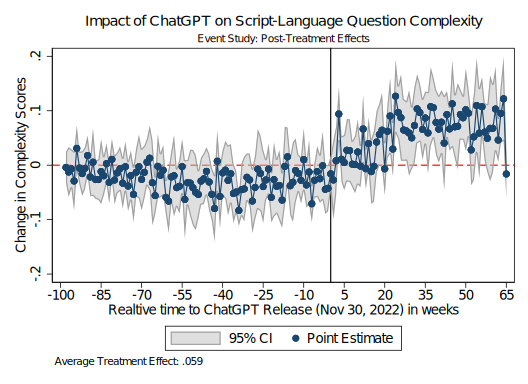
\includegraphics[width=1\linewidth]{imgs/stata/event_study_nlp.pdf}
    \caption{Event study complexity score development}
    \label{fig:cscore_event_study}
\end{figure}

\begin{table}[H]
    \centering
    \caption{Event Study: Post-Treatment Effects Over Time}
    \label{tab:csscore_event_study}
    \begin{tabular}{lccc}
    \toprule
    Time Period & Estimate & SE & 95\% CI \\
    \midrule
    Week 1-4 after treatment   & 0.310 & 0.199 & [0.121, 0.699] \\
    Week 5-12 after treatment  & 0.460 & 0.194 & [0.079, 0.841] \\
    Week 13-24 after treatment & 0.797 & 0.236 & [0.334, 1.260] \\
    Week 25-36 after treatment & 1.146 & 0.251 & [0.654, 1.638] \\
    Week 37-48 after treatment & 1.136 & 0.229 & [0.687, 1.585] \\
    Week 49-60 after treatment & 1.188 & 0.257 & [0.684, 1.693] \\
    Week 61-68 after treatment & 1.585 & 0.283 & [1.029, 2.140] \\
    \midrule
    Overall treatment effect & 1.001 & 0.064 & [0.876, 1.125] \\
    \bottomrule
    \multicolumn{4}{p{0.85\linewidth}}{\footnotesize \textit{Notes:} Results from synthetic DiD event study analysis. Estimates show the change in complexity score for Stack Overflow questions relative to the synthetic control group across different post-treatment time periods. All effects are statistically significant at the 1\% level.} \\
    \end{tabular}
\end{table}

The event study in Figure \ref{fig:cscore_event_study} reveals that the effect was immediate, with question complexity increasing sharply in the weeks following ChatGPT's release. This effect has persisted and even strengthened over time, suggesting a fundamental shift in how developers utilize Stack Overflow rather than a temporary adjustment.

\subsection{Interpretation}

These findings support our hypothesis that ChatGPT has fundamentally altered information-seeking behavior in programming communities. Developers now appear to reserve simpler questions for ChatGPT while turning to Stack Overflow for more complex programming challenges that require human expertise. The magnitude of this effect—approximately one standard deviation increase in question complexity—represents a substantial shift in the types of questions users bring to Stack Overflow.

This empirical evidence points to a complementary relationship between AI-powered assistants and human-moderated Q\&A forums, each platform serving distinct informational needs within the programming community. Stack Overflow appears to be evolving toward a repository for more complex programming questions, while more straightforward queries may be increasingly handled through interaction with large language models like ChatGPT.